% interactcadsample.tex
% v1.03 - April 2017

\documentclass[]{interact}

\usepackage{epstopdf}% To incorporate .eps illustrations using PDFLaTeX, etc.
\usepackage{subfigure}% Support for small, `sub' figures and tables
%\usepackage[nolists,tablesfirst]{endfloat}% To `separate' figures and tables from text if required

\usepackage{natbib}% Citation support using natbib.sty
\bibpunct[, ]{(}{)}{;}{a}{}{,}% Citation support using natbib.sty
\renewcommand\bibfont{\fontsize{10}{12}\selectfont}% Bibliography support using natbib.sty

\theoremstyle{plain}% Theorem-like structures provided by amsthm.sty
\newtheorem{theorem}{Theorem}[section]
\newtheorem{lemma}[theorem]{Lemma}
\newtheorem{corollary}[theorem]{Corollary}
\newtheorem{proposition}[theorem]{Proposition}

\theoremstyle{definition}
\newtheorem{definition}[theorem]{Definition}
\newtheorem{example}[theorem]{Example}

\theoremstyle{remark}
\newtheorem{remark}{Remark}
\newtheorem{notation}{Notation}

% see https://stackoverflow.com/a/47122900

% Pandoc citation processing

\usepackage{hyperref}
\usepackage[utf8]{inputenc}
\def\tightlist{}
\usepackage{gensymb}

\begin{document}

\articletype{Journal Ringing \& Migration}

\title{Using ringing data to inform a geolocator study: when and which birds to
equip?}


\author{\name{Raphaël Nussbaumer$^{a,b}$, Kirao Lennox$^{a}$, Felix Liechti$^{b}$, Colin Jackson$^{a}$}
\affil{$^{a}$A Rocha Kenya, Watamu, Kenya; $^{b}$Swiss Ornithological Institute, Sempach, Switzerland}
}

\thanks{CONTACT Raphaël Nussbaumer. Email: \href{mailto:raphael.nussbaumer@arocha.org}{\nolinkurl{raphael.nussbaumer@arocha.org}}, Kirao Lennox. Email: , Felix Liechti. Email: , Colin Jackson. Email: \href{mailto:colin.jackson@arocha.org}{\nolinkurl{colin.jackson@arocha.org}}}

\maketitle

\begin{abstract}
Light-level geolocators are increasingly used to study the migration of
small birds. Thanks to their relatively low cost, they are particularly
well-positioned to be deployed broadly across less well-financed and
understudied regions of the world, such as the Africa. A main drawback
of geolocators is the need to recapture equipped birds to retrieve the
data. Therefore, maximizing the recapture rate is critical to the
success of any geolocator study. Using the example of a geolocator study
on the coast of Kenya on Red-capped Robin-chats, this paper demonstrates
how the use of an ringing data can help optimize the deployment of
geolocators, both in terms of how many birds to set out to equip, and
when/which birds to equip to maximize recapture in the subsequent years.
We found that ringing data can help accurately estimate how many
geolocators to order and provides insights into which classes of birds
(based on age, capture history, and timing within the season) are most
likely to be recaptured.
\end{abstract}

\begin{keywords}
geolocators; ringing; red-capped robin-chat; migration; intra-african;
bird; afro-tropical;
\end{keywords}

\hypertarget{introduction}{%
\section{Introduction}\label{introduction}}

Light-level geolocators are a well-established technology used to study
bird migration. They have become popular due to their relatively low
cost and light weight, making them the only tool available to study
migration patterns of smaller birds \citep{Bridge2011}. For these
reasons, geolocators have helped advance our understanding of bird
migration on a number of levels: identifying migration routes and
wintering locations
\citep[e.g.~][]{Salewski2013, Smith2014, Liechti2015, Kralj2020},
revealing migration strategies
\citep[e.g.~][]{Adamik2016, Briedis2019, Hahn2020} and migratory
connectivity \citep[e.g.~][]{Finch2015, Prochazka2017, McKinnon2018a},
among others. Geolocators bear strong potential to uncover long-distance
Afro-tropical migration patterns, many of which remain still largely
unknown
\citep[e.g.~][]{Benson1982, Bennun2000, Cox2011, Bussiere2015, Nwaogu2016, Osinubi2018}.
As habitat destruction and climate change accelerate and adversely
affect migrant birds, it is becoming urgent to better understand these
patterns to effectively protect these migratory bird populations
\citep[e.g.~][]{Simmons2004, Sekercioglu2010, Sekercioglu2012, Vickery2014}.
Geolocators are instrumental in helping us gain understanding of
migration routes, timing, triggers and variability, as well as
identifying breeding, wintering and stopover sites to protect. Thanks to
their low price, geolocators are particularly well-suited to projects
with limited budgets. However, geolocators are not without drawbacks.
The tags must be retrieved to recover data, harnesses can fail, bird
survival might be impacted, latitudinal precision can be relatively
poor, and the data analysis can be difficult and prone to errors. With
the increasing number of studies using geolocators, these challenges
have been partially addressed. Increased experience with this technology
has helped improve survival rates through minimum relative load and
non-elastic harness technology
\citep[e.g.~][]{Streby2015, Weiser2015, Brlik2020}. Data analysis has
also become more accessible and accurate (e.g.~\citet{Lisovski2012};
\citet{Lisovski2020}) and common pitfalls in analysis have been
discussed \citep[e.g.~][]{Fudickar2012, Lisovski2012, Lisovski2018}.
Finally, more recent geolocators also measure temperature, air pressure
and bird activity, providing further precision in geolocation and
additional research opportunities
\citep[e.g.~][]{Meier2018, Liechti2018, Dhanjal-Adams2018, Sjoberg2018, Jiguet2019, Briedis2020}.
Despite this progress, geolocator studies still need to be carefully
planned (in terms of field time, research questions, sample size etc.)
to improve the recapture rate of birds in subsequent years. In this
study, we present an example of one geolocator study carried out on two
Afro-tropical migrants in Kenya. This study will demonstrate how
pre-deployment analysis using an existing ringing database can help
optimize the deployment of geolocators. We focus on two questions in
particular: (1) how many birds can we expect to capture during a full
season for a given ringing schedule and (2) how can we maximize bird
recapture by equipping specific classes of birds (e.g.~sex, age) during
specific periods of the year?

\hypertarget{materials-and-methods}{%
\section{Materials and methods}\label{materials-and-methods}}

\hypertarget{ringing-site-and-database}{%
\subsection{Ringing site and database}\label{ringing-site-and-database}}

The A Rocha Kenya Conservation Centre is located on the coast of Kenya
and in the middle of the Northern Zanzibar-Inhambane Coastal Forest
Mosaic ecoregion (3\degree 22'36.3``S 39\degree 59'16.9''E). This region
is recognized for its high biodiversity value \citep{Marris2010} yet
faces increasing habitat fragmentation due to the expansion of
agriculture and charcoal burning \citep{Burgess2000CoastalFO}.

The Conservation Centre is located on a residential coastal scrub/forest
that has benefited from limited habitat change over the last 50 years
\citep{Alemayehu2016}, in the effort to preserve the ecosystems for
tourism purposes. Mist nets are placed in a nature trail that runs
through a small patch of forest managed by the Conservation centre.

In this study, we use the ringing dataset from ringing sessions
conducted regularly from 2002 to present. Up to early 2019, the dataset
consists of 3372 entries of 2532 rings covering 96 species collected
during 317 sessions. The ringing effort presents some temporal
variability, as well as variability in the metadata recorded (see SM1).
In general, sessions start at sunrise (M=06:12 ; SD=00:14) and last
until bird activity slows down (session duration M=04:08 ; SD=01:01)
(see Figure 7 in SM1). On average, a total of 154.3424658 m
(SD=51.5159682 m) of nets were used. Descriptive notes on weather
conditions were also included, and later classified according to their
expected influence on the capture rate (none, little, large). We
manually checked extreme values in the dataset and removed those that
could not be verified.

In addition, we also present the ringing data of 2020, when the
geolocators were first deployed. We did not include this data in the
fitting of the models but rather used it for comparison and discussion
purposes.

In this case study, geolocators were placed on Red-capped Robin-chats
Cossypha natalensis (RCRC), a terrestrial thrush wintering in the area
from April to October, to uncover their summering site and migration
routes (Nussbaumer \& Jackson, 2020). RCRC are known to hold territory
on their wintering sites and show site fidelity (C. Jackson, personal
communication), thus making them an ideal candidate for a geolocator
study.

\hypertarget{capture-model}{%
\subsection{Capture model}\label{capture-model}}

An early question in the planning stage is how many geolocators to
deploy and therefore order. To answer this, it is important to
accurately estimate the number of individuals that can realistically be
captured per ringing season. Geolocators are configured to collect data
for a single year, and therefore cannot be kept for future studies.
Overestimating the individuals captured would thus result in wasting
devices, while underestimating would result in missed opportunities. The
estimation also directly influences the ringing effort planned
(i.e.~number of sessions, duration of session, number of nets etc). To
address this question, we followed a three-step process described below.

In the first step, we modelled the number of RCRC captured per session
using a generalized additive model (GAM), assuming the number of
captures follows a Poisson distribution. The predictor variables tested
in the model are (1) year (2) day-of-year, (3) duration of the session,
(4) total length of nets, (5) starting time and (6) weather conditions.
To overcome the lack of sufficient data for the duration, start time and
length of nets, we used multiple imputation methods by chained equations
\citep{Azur2011} to generate 30 sets of data without any missing values.
For each of these sets, a GAM model was fitted.

In the second step, we addressed the problem that RCRC can only be
equipped once a year. A first approach tested was to model the count of
new birds (i.e., birds that have not yet been captured in the same year)
rather than the total number of birds. However, this count depends on
how many RCRC have already been equipped earlier in the year. Instead,
we preferred to model the probability that a bird captured was not
already captured in the same year. This probability is modelled with a
Generalized Linear Model (GLM) using a binomial family and a single
explanatory variable consisting of the total number of RCRC captured in
the year.

In the third step, we used the two models above to predict the number of
RCRC that can be captured over one year. This number is estimated from
the prediction of the models under various ringing scenarios. The
default scenario for our ringing season of 2020 is to ring every week
for 4 hours using 156m of nets. Using the first model and this
information, we can estimate the total number of RCRC that would be
captured in the season. Knowing how many birds have been captured, we
used the second model to predict how many unique RCRC can be equipped
along the year by multiplying the number of captures by the probability
of each individual being a new bird. Finally, assuming that the sessions
are independent conditional to the model, we estimate the total number
with a cumulative sum over the year.

This approach was performed under different scenarios where we modified
the number of ringing sessions, total length of nets, and duration of
ringing session. The default scenario includes 4 hr-ringing sessions
every 10 days with 156 m of nets. We tested the influence of increasing
the duration of the ringing sessions to 6 hrs and the length of nets to
225 m. In addition, we tested an optimized ringing schedule where more
ringing sessions are held during the peak passage. Finally, we also
compared the actual number of RCRC captured in 2020 with the prediction
of our model using the exact session durations and lengths of nets.

\hypertarget{recapture-model}{%
\subsection{Recapture model}\label{recapture-model}}

Data collected by geolocators can only be retrieved if the equipped bird
is recaptured in the following years. Consequently, to optimize the
study it is essential to equip those birds that are most likely to be
recaptured. Here too, the ringing database can inform this decision, in
this case by providing the recapture rate of a bird as a function of the
date of equipping but also of the age and weight of the bird. Using this
information, the ringer can make an informed decision about whether or
not to equip a captured bird. This decision should also account for the
total number of geolocators available and the number of sessions left.

In this study we looked at two parameters: the time of year and the age
class (adult or juvenile). The recapture probability is estimated by
modelling the binomial response of whether a captured bird will be
recaptured in the following years: we consider that an individual is
recaptured if the bird has been recaptured at least once in any of the
following years, and this is independent from whether it was already
captured in the past. We modelled the count of adults and juveniles per
session separately to reveal the influence of age on recapture rates.
The weight of the bird was left out of the model as it showed little to
no effect on the recapture rate (see Figure 10 in SM3). Additionally, we
also compare the recapture rate for RCRC captured for the first time and
those which have already been equipped.

All computation was performed on R \citep{team2013r}, using the MCGV
package \citep{wood2017generalized} for GAM, and the Mice Package
\citep{Buuren2011} for the imputation.

\hypertarget{results}{%
\section{Results}\label{results}}

\hypertarget{capture-model-1}{%
\subsection{Capture model}\label{capture-model-1}}

A GAM model was fitted to the data to model the number of RCRC captured
for each session. After testing several parametrizations of the model
(see SM2), we retained the capture model that included a smooth function
of day-of year, year and total length of a linear function of the
duration of the session. The fitted model for the default case (156 m of
nets and session duration of 4 hrs) together with the raw counts data is
illustrated in Figure 1. The model fits a typical migrant phenology
curve, with a steep increase in the numbers in May, peaking in early
June with almost three RCRC per session. The second peak of returning
birds in mid-September is much smaller with only 1.5 birds/session on
average. The counts of 2020 show an early arrival of birds (peak in
second half of May), but overall, within the range of a typical year.

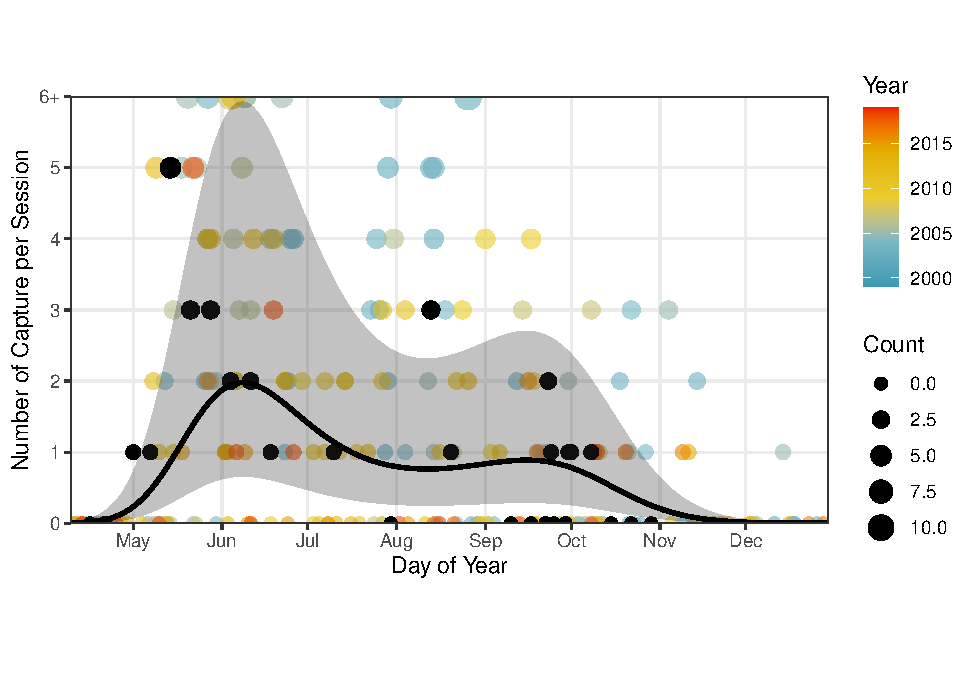
\includegraphics{manuscript_files/figure-latex/seasonal-variation-counts-1.pdf}
We modelled the probability of recapture within a year to extract the
number of unique birds captured during a single year (Figure 2). As the
cumulative number of RCRC captured increases, so does the recapture rate
and consequently, the probability of being a new bird decreases from
around 100\% for the first bird to 60-70\% after 40 RCRCs have been
captured in the year. Note that this approach can only reliably estimate
the probability up to a maximum of around 40 RCRCs captured in a year.

\begin{figure}
\centering
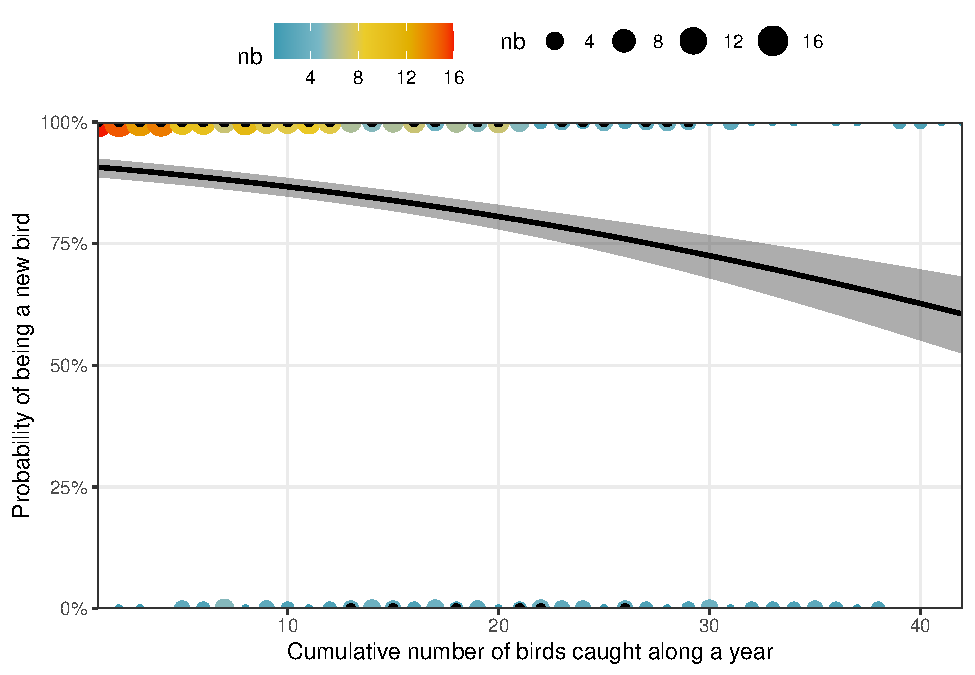
\includegraphics{manuscript_files/figure-latex/prob-new-bird-1.pdf}
\caption{The probability of capturing a new bird (i.e., a bird not yet
captured in the current year) as a function of the number of RCRC
capture increases. The colour and size of the points indicate the number
of occurrences in the dataset that the nth bird caught in a year had
already been caught during the year (bottom, old bird, 0\%) or the first
time it was caught this year (top, new bird, 100\%). The line shows the
fitted model of the probability that a bird is a new bird as a function
of its rank of capture.}
\end{figure}

\begin{figure}
\centering
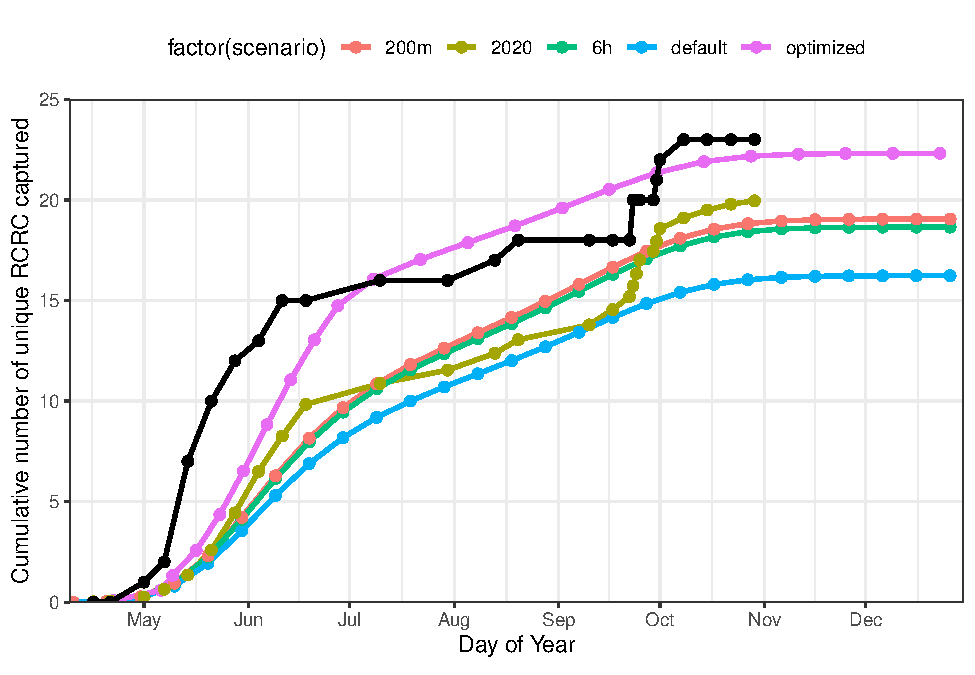
\includegraphics{manuscript_files/figure-latex/total-rcrc-captured-1.pdf}
\caption{Model predictions of the total unique RCRC caught along a year
following different scenarios. The default scenario consists of 4hr
ringing sessions using 156m of nets every 10 days. `6h' and `225m' are
modifications of the default scenario, and `optimized' increases the
number of sessions (to every week) during the peak passage (mid-May --
July) and decreases them (to every 2 weeks) during the rest of the year.
Finally, using the exact date, duration, and net length used in 2020,
the model prediction `2020 model' can be compared to the actual data
(`2020 data').}
\end{figure}

Five different scenarios of ringing were modelled to estimate the total
number of unique RCRC captured along the year in Figure 3. Compared with
the total number of birds caught at the end of year with the default
scenario (16), increasing the duration of ringing sessions by two hours
(`6hr') or adding 44m of additional nets (`200m') results in only three
more birds caught (19). However, the optimized scenario yields many more
birds, with a total of 22 birds captured in fewer number of sessions (31
instead of 37).

In 2020, 27 ringing sessions were held with 156 m of mist nets, with an
average duration of 3:45 (SD: 0:59). As of the 1st of November, a total
of 29 RCRC were capture from 23 unique individuals. For the exact same
information, the model predicted an expected total of 23 RCRC from 20
individuals.

\hypertarget{recapture-model-1}{%
\subsection{Recapture model}\label{recapture-model-1}}

Over the 161 unique RCRC individuals captured in the dataset, 67 (42\%)
were recaptured at least once (including recapture the same year). When
considering the 301 capture events (including same individuals), the
general recapture rate increases to 47\%. However, looking at captures
with recapture in any subsequent year, the recapture rate is 30\%. In
the rest of the study, we employ the latter definition of recapture rate
to eliminate intra-season recaptures and consider only recaptures in
subsequent years, when geolocators can be retrieved.

In general, adults show a slightly higher recapture rate (34\%) than
juveniles (27\%). When modelled over the day of year (Figure 4a), the
recapture rate in subsequent years shows that birds equipped later in
the year are twice as likely to be recaptured, with a recapture rate
increasing from 25\% to almost 50\%. Separating adults from juveniles
allows us to identify further trends. The increase in juveniles'
recapture rate is not significant. By contrast, adults show a clear
increase from May to August, before stabilising from September to
October. Modelling the number of captures of adults and juveniles
(Figure 4b), we observe an earlier arrival of juveniles (late May vs
early June for adults) and earlier departure in August, while adults
show a second peak early October.

Finally, a RCRC which has already been captured in the past has a higher
recapture rate (36\%) compared to a bird without a ring (24).

\begin{figure}
\centering
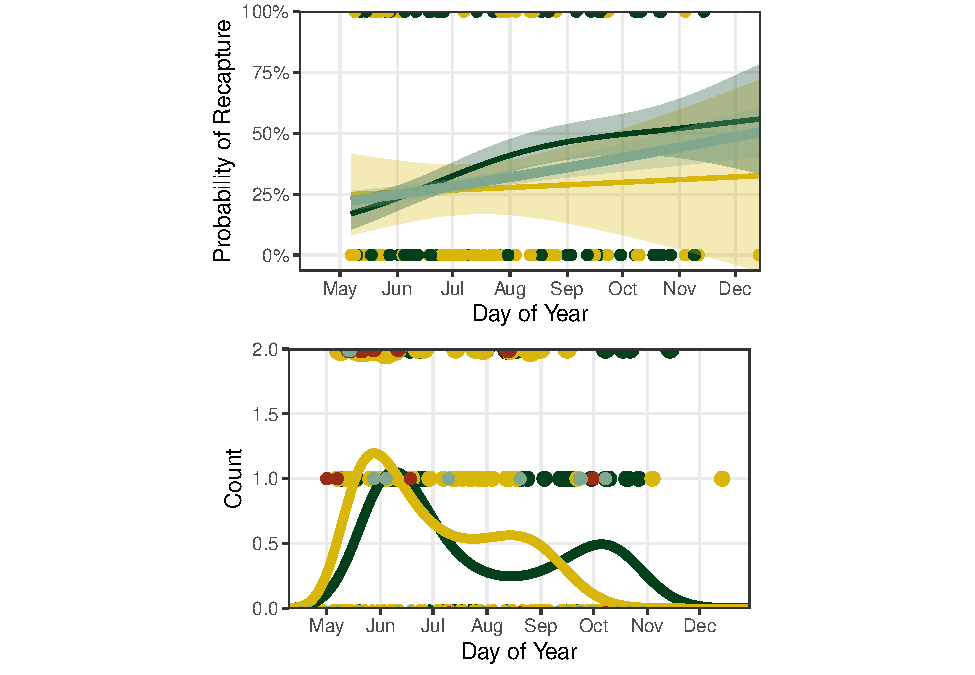
\includegraphics{manuscript_files/figure-latex/recapture rate-1.pdf}
\caption{Comparison of adult (green) and juvenile (yellow) trend in (a)
recapture rate in subsequent year and (b) number of captures per session
throughout the year.}
\end{figure}

\hypertarget{discussion}{%
\section{Discussion}\label{discussion}}

In this paper, we provide an example of how a ringing dataset can inform
the design and planning of a geolocator study.

\hypertarget{how-many-captures}{%
\subsection{How many captures?}\label{how-many-captures}}

The method outlined above allows us to estimate the total number of
individual birds that can be captured and equipped with geolocators
during a single season while accounting for the ringing schedule (number
of sessions along the year, length of nets, and session duration).

In addition, the capture model provides practical information for
planning ringing sessions with the goal of maximizing the number of RCRC
captured. Increasing the duration of ringing sessions from four to six
hours and increasing the length of nets only slightly improves the total
number of RCRC captured. This is explained by the fact that RCRC are
mostly active in the early hours of the day, and that additional nets
are placed in successively sub-optimal habitats. By contrast, increasing
the number of sessions as well as selecting the right time of year
significantly increases the number of captures. This model allows us to
identify an optimal ringing schedule, with the highest number of RCRC
captured (22 vs 16) for the fewest ringing sessions (31 vs 37) (Figure
3).

In 2020, the initial plan was to ring at minimum every two weeks, and
every week during peak passage (from May to early June and from late
August to October). Following an earlier and simpler capture model (not
accounting for annual trends or recapture rates), we expected to capture
a total of 30 individuals. Because of uncertainties surrounding the
first deployment year, we conservatively requested 15 geolocators. This
was meant to allow for flexibility in learning how to equip, and how to
select which birds to equip and when throughout the year.

\hypertarget{how-to-improve-recapture-rates}{%
\subsection{How to improve recapture
rates?}\label{how-to-improve-recapture-rates}}

For the geolocator study to be successful, not only do we need to
maximize the number of birds equipped (with minimal ringing effort), but
also optimize their recapture (i.e.~number of geolocators retrieved). We
analysed the recapture data for two parameters: age class, and capture
date in the year.

Equipping individuals which have already been captured before has the
largest influence on recapture, improving the probability of recapture
by 1.5 times (36\% vs 24\%). Moreover, equipping adults provides better
probability of recapture than juvenile (34\% vs 27\%). This is
especially true for adults captured later in the year, which suggest
that these adults are holding territories on site and thus coming back
every year.

This information was included in our deployment by equipping all adults,
especially if they had already been captured. While waiting for
July/August seemed preferable to increase the recapture rate, the number
of birds captured decreases strongly in this period. In addition, to
learn more about the age difference patterns observed in the ringing
data and to test the hypothesis of variable departure/arrival dates
based on age, we decided to equip both juveniles and adults. In
practice, we limited ourselves to the deployment of 6 RCRC up to
mid-June (out of the 15 available), when juveniles were more common
(74\%), in order to have enough geolocators in July and August, when we
were able to equip more adults (53\%). Model validation, limitation and
extension

We can loosely validate the capture model results with the actual data
collected in 2020, though caution is needed as this represents only a
single year. The number of RCRC captured in 2020 is comparable to the
model estimate, albeit slightly higher. The arrival date proved to be
earlier than the average and the numbers appeared to be higher than
average at the beginning of the season. This could be due to a
particularly good breeding season (many juveniles caught during this
period) and/or affected by the playback used near the nets (not done in
previous years).\\
The approach followed in this paper contains some limitations. Firstly,
we considered a recapture as when a bird was captured again in any
subsequent year of the initial capture. However, for a geolocator study,
the recapture needs to happen within the duration of the study. The
recapture rate of the full dataset (30\%) reduces to 19\% when
considering only recaptures happening exactly the following year, 26\%
for the following 2 years, and 28\% for the following 3 years. This
suggests that we should keep ringing for at least 2 seasons after
captures to benefit from a maximum of geolocator data. Secondly, by
using recapture data from the ringing database as a proxy for recaptures
involving geolocators, we ignore the effect of geolocators on survival
rate (or site fidelity). There have been instances where geolocators
have had an impact on survival, thus leading to lower recapture rates
than for rings (unknown effect of ring).

One last question remained to be answered to finalise the geolocator
study, and that was when nets should be put up in the following year to
attempt to recapture birds. To answer that question, we simply verified
that the probability of capturing a recapture (i.e.~a bird captured
before) or a new bird is the same throughout the year. We verified that
this is the case in Figure 9 in SM3, thus suggesting that one simply
needs to follow the result of how to maximize captures to also maximize
recaptures.

Although the model and results of this study are tailored for the
specific case of RCRC on coastal Kenya, the application of this
methodology can be extended to other situations where ringing data are
available for a study site. In general, our methodology is only
applicable for cases where the deployment of geolocators is performed
with the same technique (e.g.~mist net, nest trap, spring nest trap) and
context (e.g.~place, time, general ringing effort) as the ringing
database. In this study, we carried out analyses comparing only adults
and juveniles, because it is not possible to determine the sex of a bird
in hand. The same analysis can be performed on any class of bird
identified by ringers (sex, molt stage, breeding status, subspecies).

\hypertarget{conclusion}{%
\section{Conclusion}\label{conclusion}}

The use of geolocators to study the migratory patterns of smaller birds
has accelerated in recent years, offering an affordable solution to
better understand, or uncover yet unknown migration routes and sites.
This is of particular relevance for Afro-tropical migrants, many of
which are still widely understudied and poorly understood, often due to
lack of adequate research funding. Along with an increased collective
experience in geolocator deployment, the design of studies and analysis
of retrieved data has considerably improved. To further contribute to
this effort, this study explores avenues for optimizing the deployment
of geolocators, in terms of how many, when, and which birds to equip
throughout a ringing season in order to maximize re-capture and
subsequent retrieval of data. Using the case study of a geolocator study
on Red-capped Robin-chats, we exploit the potential of an existing
ringing database to inform these questions and design a study. This
initial research opens the door for further applications of ringing data
to inform geolocator studies.

\hypertarget{supplementary-materials}{%
\section{Supplementary Materials}\label{supplementary-materials}}

\hypertarget{sm1-data-extends}{%
\subsection{SM1 Data extends}\label{sm1-data-extends}}

The ringing sessions are relatively well-spread throughout the year
(y-axis in Figure 6), although with a slightly higher intensity in
March-April than June-July or December-January. The distribution is more
heterogenous when comparing different years (x-axis in Figure 6): there
is very good coverage between 2003 and 2007, variable from 2008 to 2012,
and relatively correct since then.

\begin{figure}
\centering
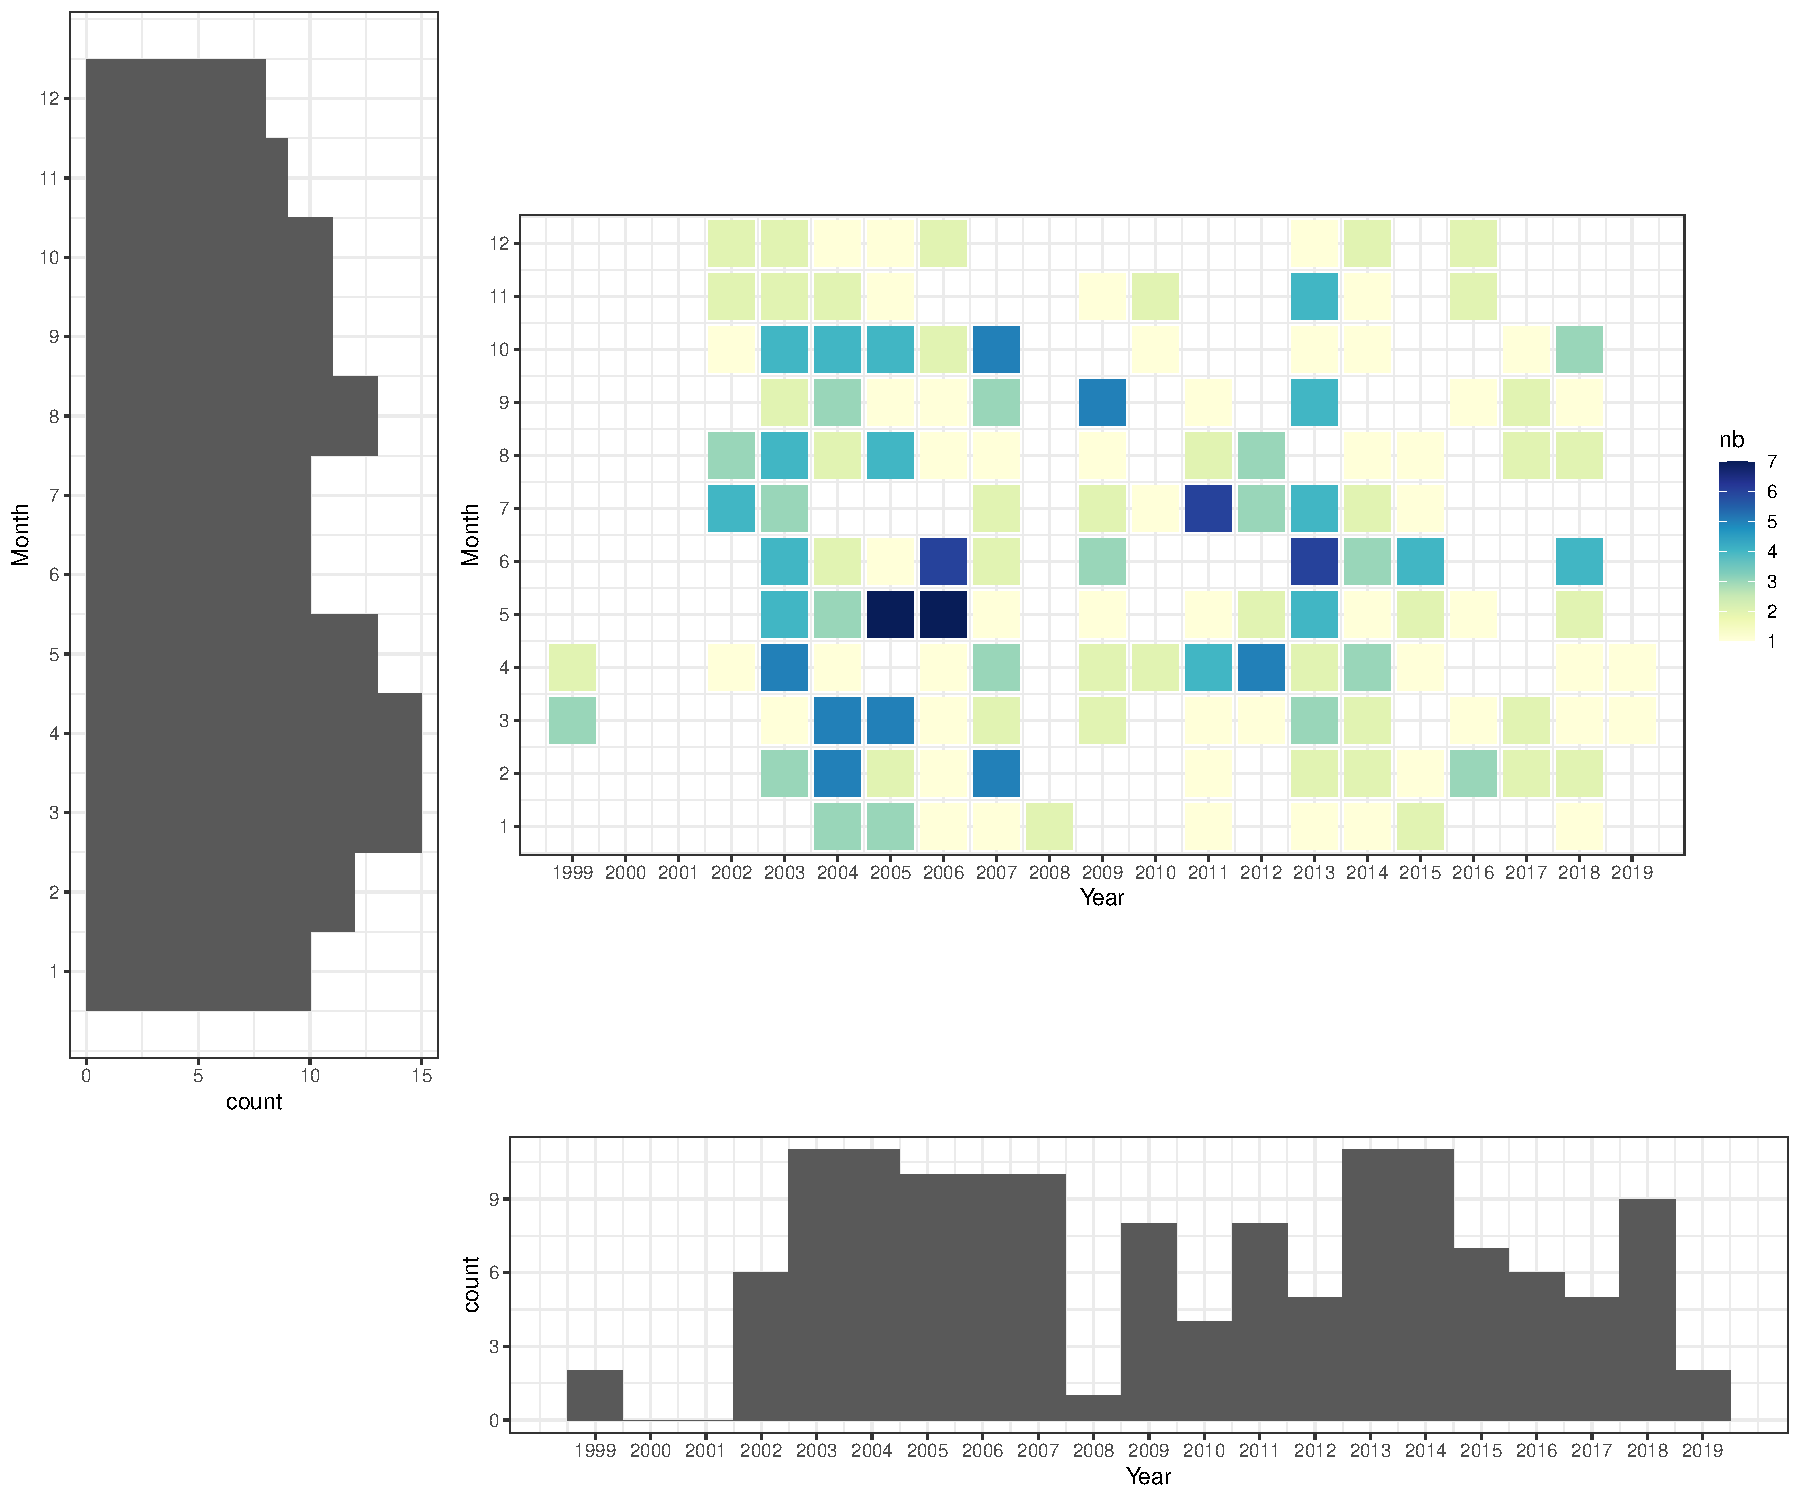
\includegraphics{manuscript_files/figure-latex/unnamed-chunk-8-1.pdf}
\caption{Distribution of the ringing sessions according to year and
month. Colour scale indicates the number of ringing sessions.}
\end{figure}

Additional information for each session was available for some sessions:
start time (data available for 74\% of the sessions), closing time
(39\%), sum of net lengths (23\%), weather conditions (45\%).

\begin{figure}
\centering
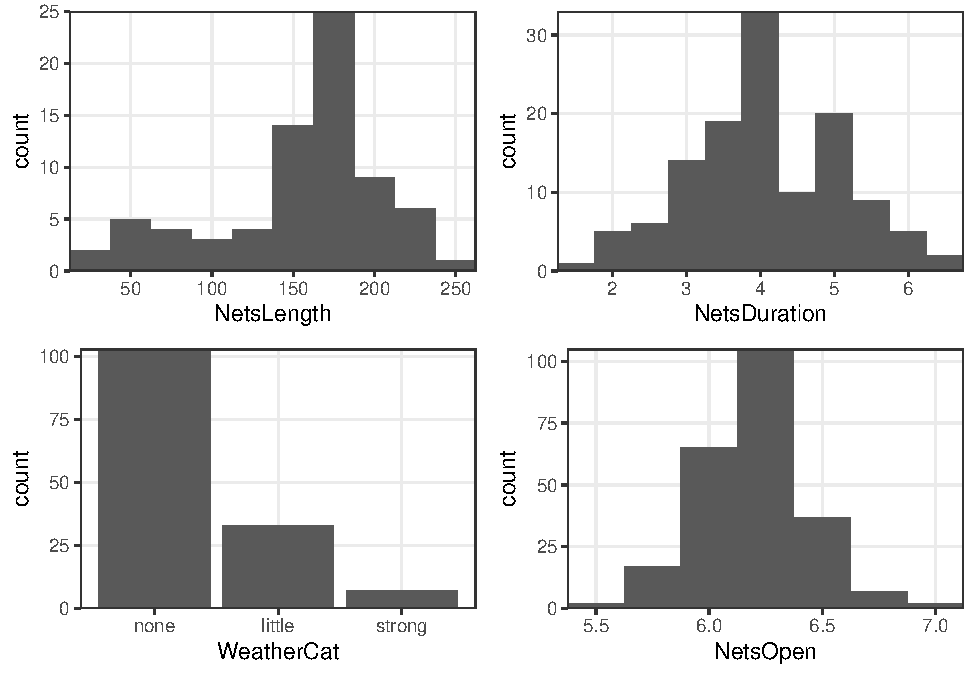
\includegraphics{manuscript_files/figure-latex/unnamed-chunk-9-1.pdf}
\caption{Histograms of the metadata collected for each ringing session
(N=317) of (a) total length of nets (N=73), (b) duration of ringing
session (N=124), (c) weather category (N=143) and (d) time of session
start (N=235).}
\end{figure}

\hypertarget{sm2-capture-model}{%
\subsection{SM2 Capture Model}\label{sm2-capture-model}}

The GAM of the count (i.e.~number of RCRC captured per session) was
tested with (1) year (2) day-of-year, (3) duration of the sessions and
(4) starting time, (5) total length of nets and (6) weather. We first
tested a GAM smoothing for each variable separately to analyse its
effect (Figure 8). a) Year (Figure 8a). A general decline in the overall
number of birds is observed over the 20 years of the dataset. It was
included as a smoothing term. b) Day-of-year (Figure 8b). Day-of-year
has a strong influence on the number of captures and varies
non-linearly. This variable is thus included in the model as a smoothing
term. c) Duration (Figure 8c). The duration of the session computed as
the difference between closing time and opening time shows a positive
correlation with the number of captures. It is thus included in the
model as a linear term. d) Net opening time (Figure 8d). The fit of the
opening time seems to indicate a higher capture rate for sessions
starting later. This relationship is contrary to common knowledge and
considered non-meaningful. It is thus not retained for the model. e) Sum
of net lengths (Figure 8e). Between 50 and 200m, the fit shows an
increase of captures as the total length of the nets increases. Yet,
above 200m, the fit shows a stabilisation of the count. This is
explained by the fact that the nets added above 200m are located in
habitats which are not ideal for RCRC and thus do not contribute to an
increase in capture. This term is included as a smoothing term. f)
Weather categories (Figure 8f). The weather categories do not show a
clear pattern and are thus not included in the model. The retained model
was
\texttt{Count\ \textasciitilde{}\ s(DayOfYear)\ +\ s(Year)\ +\ Duration\ +\ s(SumNetLength)}.

\begin{figure}
\centering
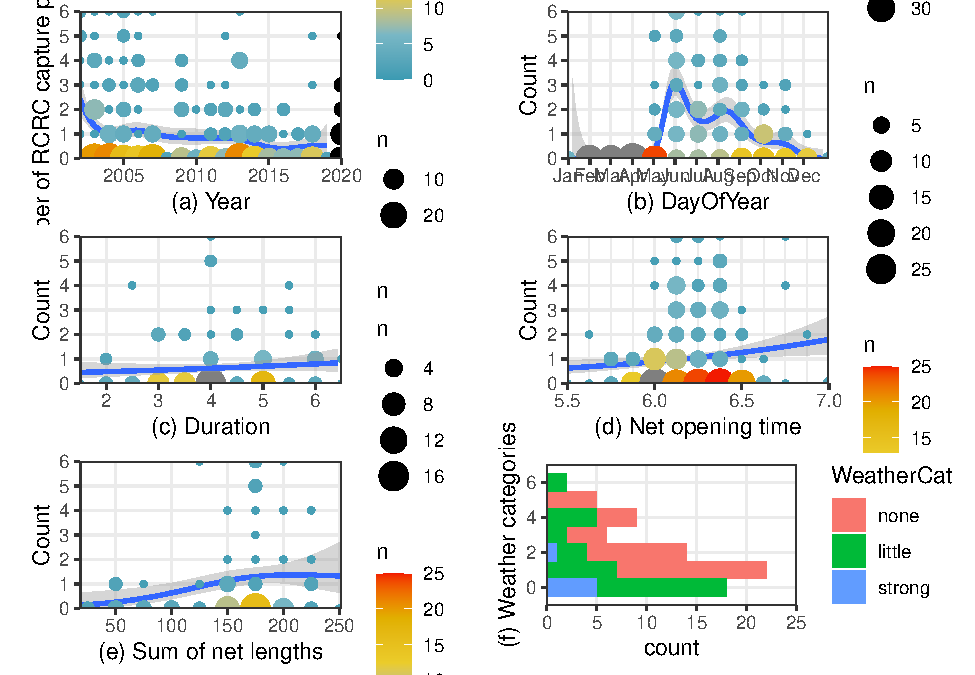
\includegraphics{manuscript_files/figure-latex/unnamed-chunk-10-1.pdf}
\caption{Number of RCRC captured by session as a function of (a) total
length of nets, (b) duration of ringing session, (c) weather category
and (d) time of session start. The red line with shaded area is a
smoothed curved fitted on the data (GAM or GLM)}
\end{figure}

\begin{verbatim}
## 
## Family: poisson 
## Link function: log 
## 
## Formula:
## Count ~ s(Year) + s(DayOfYear) + NetsDuration + NetsLength
## 
## Parametric coefficients:
##               Estimate Std. Error z value Pr(>|z|)    
## (Intercept)  -5.651480   0.736007  -7.679 1.61e-14 ***
## NetsDuration  0.195472   0.040562   4.819 1.44e-06 ***
## NetsLength    0.006965   0.001004   6.934 4.09e-12 ***
## ---
## Signif. codes:  0 '***' 0.001 '**' 0.01 '*' 0.05 '.' 0.1 ' ' 1
## 
## Approximate significance of smooth terms:
##                edf Ref.df Chi.sq p-value    
## s(Year)      8.419  8.859  148.2  <2e-16 ***
## s(DayOfYear) 8.891  8.991  187.8  <2e-16 ***
## ---
## Signif. codes:  0 '***' 0.001 '**' 0.01 '*' 0.05 '.' 0.1 ' ' 1
## 
## R-sq.(adj) =  0.488   Deviance explained = 57.8%
## UBRE = 0.073988  Scale est. = 1         n = 634
\end{verbatim}

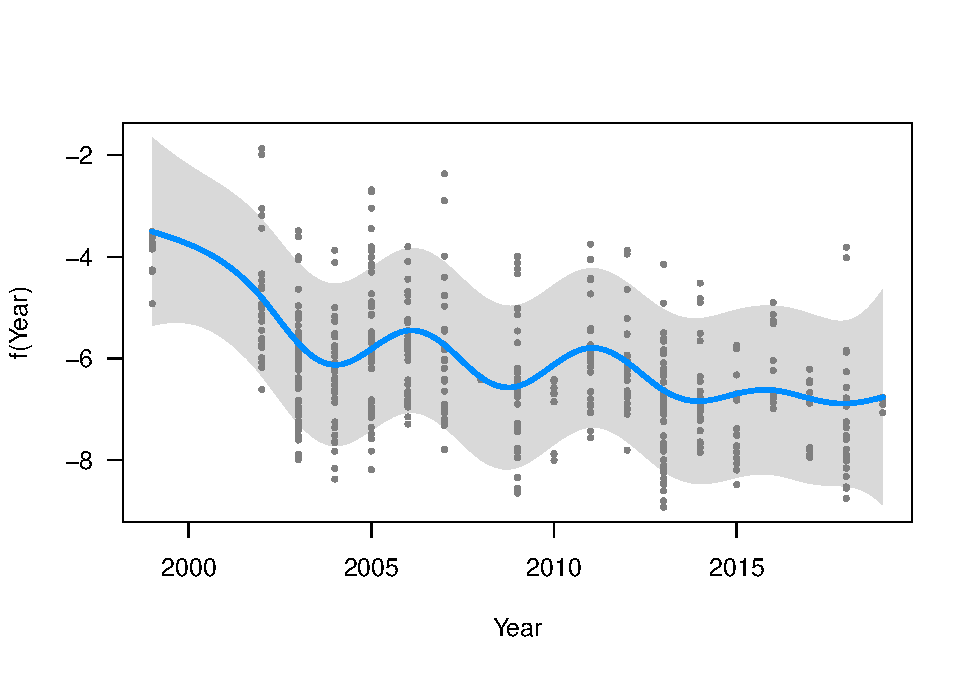
\includegraphics{manuscript_files/figure-latex/unnamed-chunk-11-1.pdf}
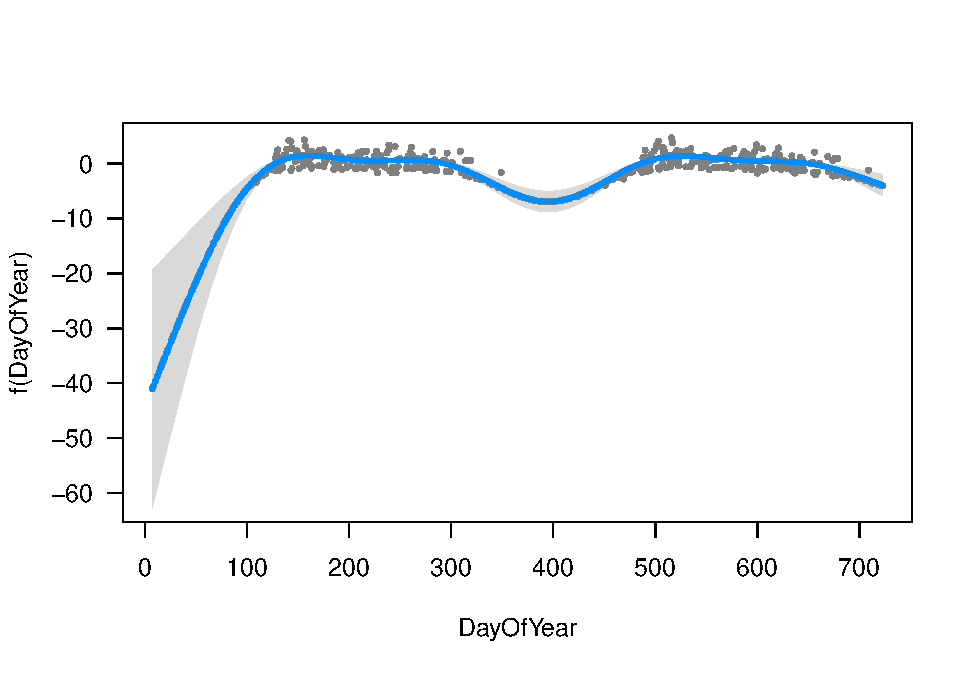
\includegraphics{manuscript_files/figure-latex/unnamed-chunk-11-2.pdf}
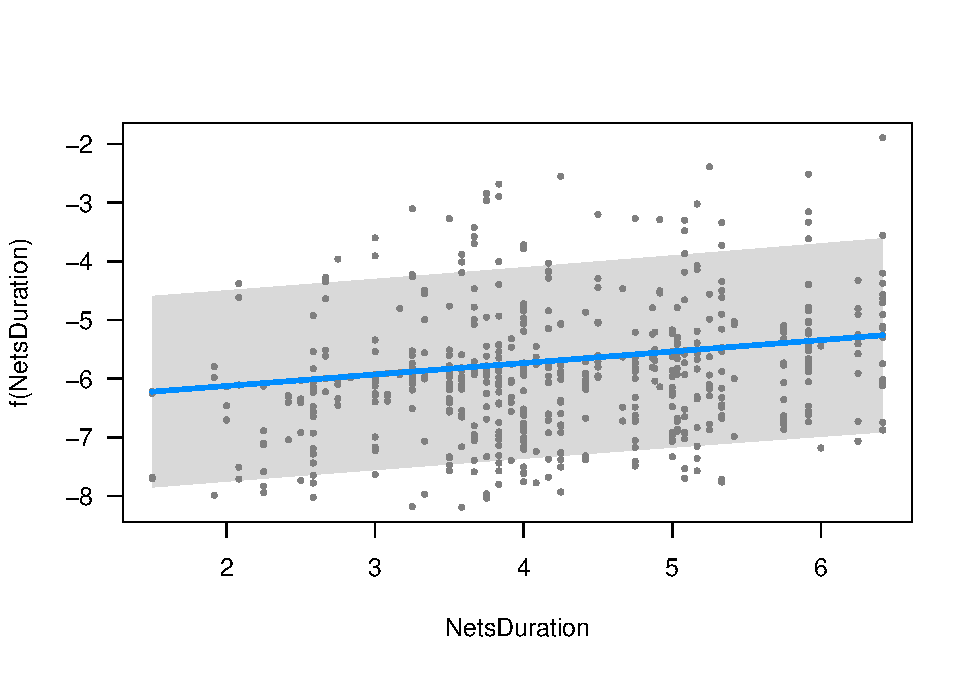
\includegraphics{manuscript_files/figure-latex/unnamed-chunk-11-3.pdf}
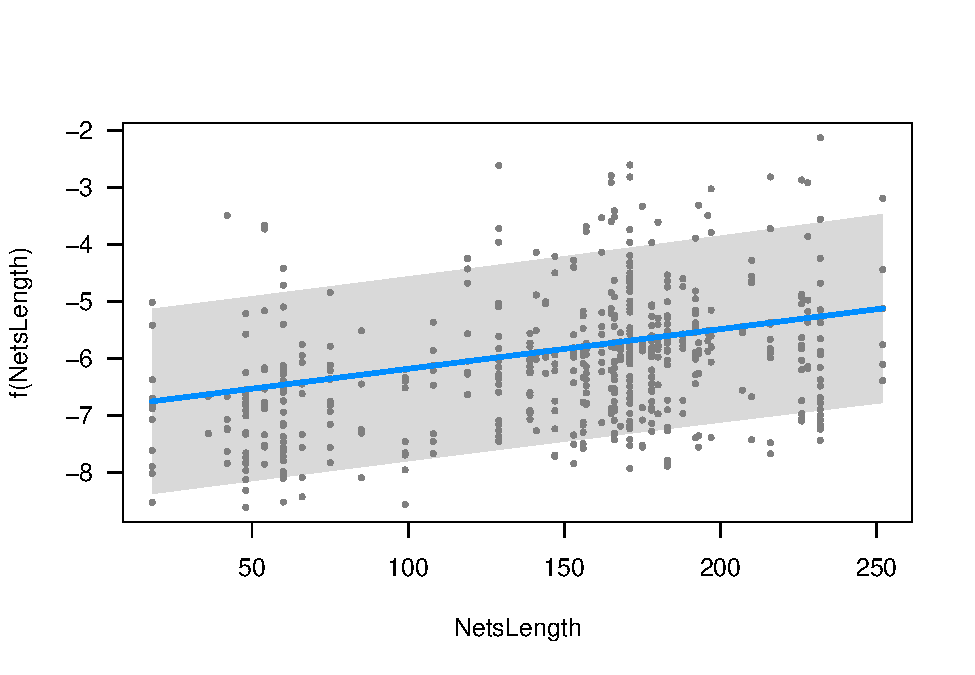
\includegraphics{manuscript_files/figure-latex/unnamed-chunk-11-4.pdf}

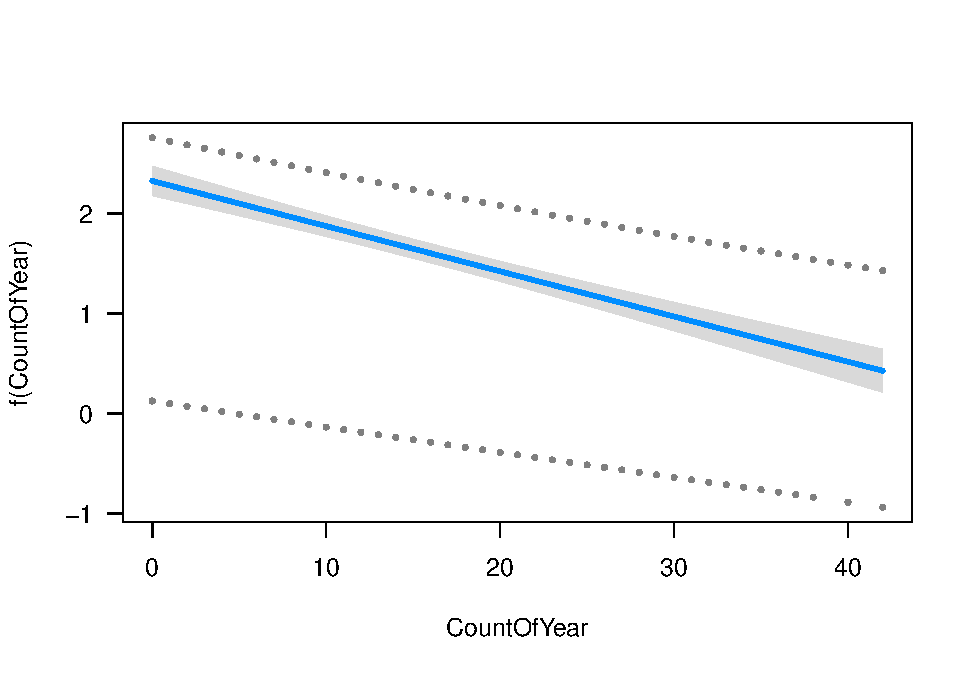
\includegraphics{manuscript_files/figure-latex/unnamed-chunk-12-1.pdf}

\begin{verbatim}
## 
## Call:
## glm(formula = isFirstOfYear ~ CountOfYear, family = "binomial", 
##     data = dmf)
## 
## Deviance Residuals: 
##     Min       1Q   Median       3Q      Max  
## -2.2001   0.4315   0.4603   0.5688   1.0015  
## 
## Coefficients:
##             Estimate Std. Error z value Pr(>|z|)    
## (Intercept)  2.32700    0.07587   30.67   <2e-16 ***
## CountOfYear -0.04519    0.00372  -12.15   <2e-16 ***
## ---
## Signif. codes:  0 '***' 0.001 '**' 0.01 '*' 0.05 '.' 0.1 ' ' 1
## 
## (Dispersion parameter for binomial family taken to be 1)
## 
##     Null deviance: 2858.4  on 3371  degrees of freedom
## Residual deviance: 2713.4  on 3370  degrees of freedom
## AIC: 2717.4
## 
## Number of Fisher Scoring iterations: 4
\end{verbatim}

\hypertarget{sm3.-recapture-model}{%
\subsection{SM3. Recapture model}\label{sm3.-recapture-model}}

\begin{figure}
\centering
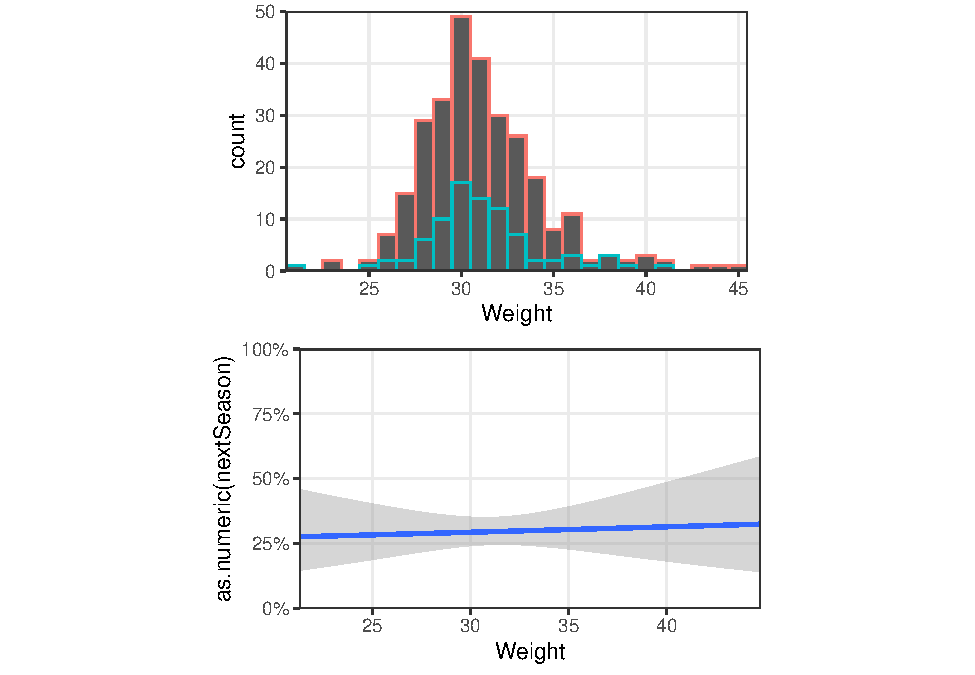
\includegraphics{manuscript_files/figure-latex/unnamed-chunk-13-1.pdf}
\caption{Histograms of the weight of RCRC recaptured in a following year
and those not recaptured, together with the model fit. The uncertainty
of the model shows that weight has an unclear influence on the recatpure
rate.}
\end{figure}

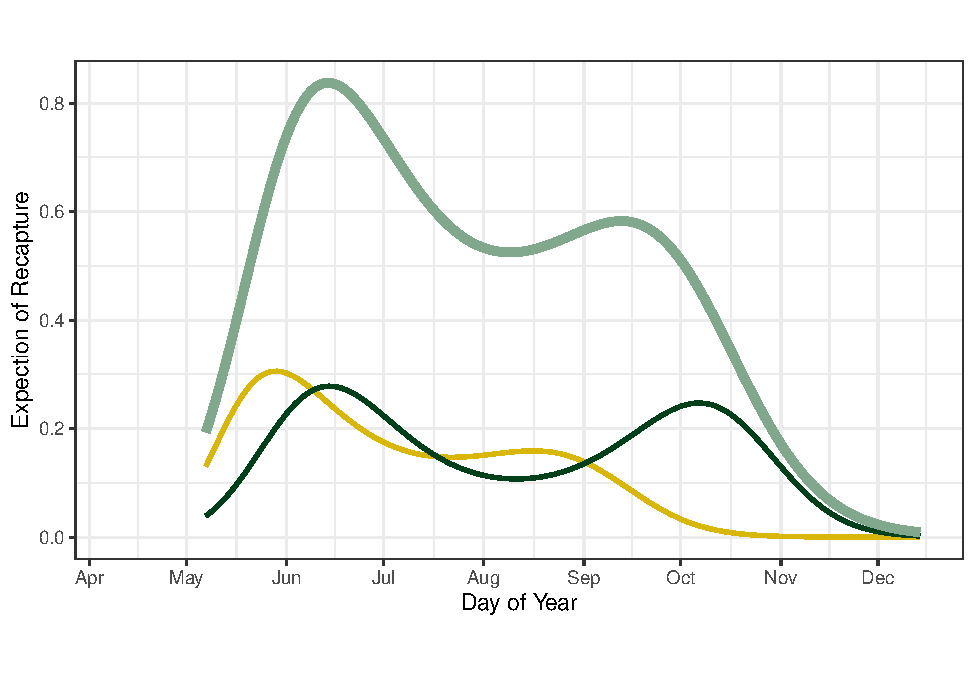
\includegraphics{manuscript_files/figure-latex/expection-1.pdf}
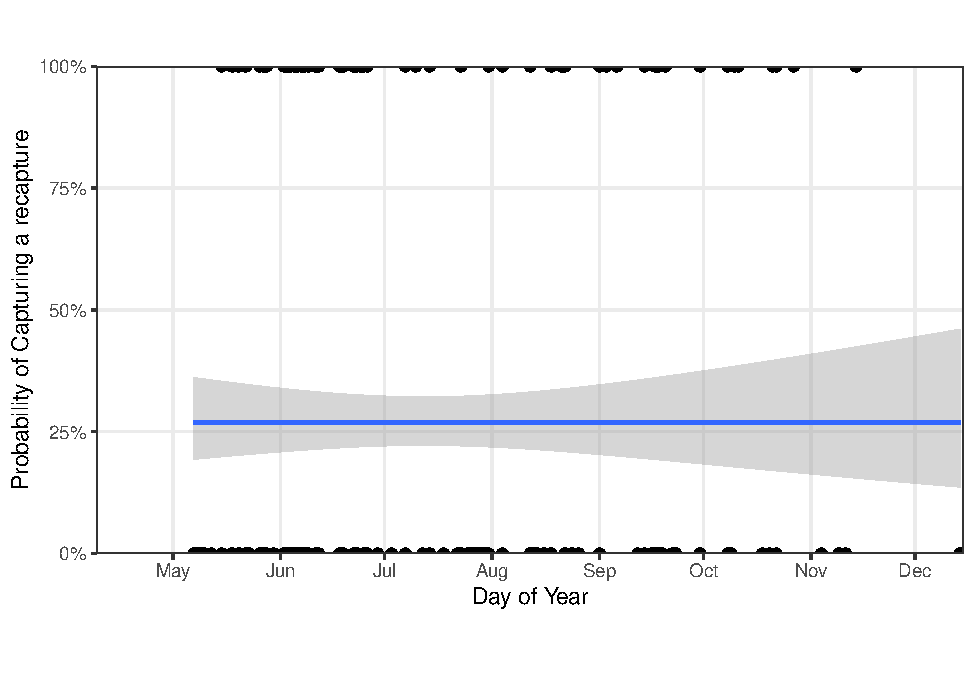
\includegraphics{manuscript_files/figure-latex/capture vs recapture-1.pdf}

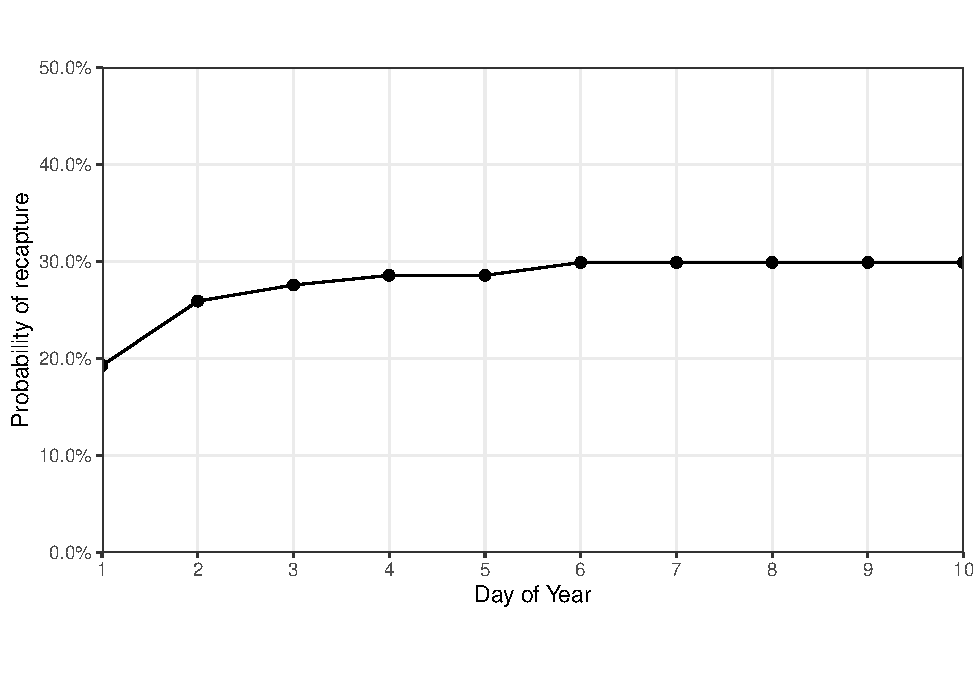
\includegraphics{manuscript_files/figure-latex/unnamed-chunk-14-1.pdf}

\hypertarget{acknowledgements}{%
\section*{Acknowledgements}\label{acknowledgements}}
\addcontentsline{toc}{section}{Acknowledgements}

This work was supported by a grant from the Swiss Ornithological
Institute. We thank A Rocha Kenya for providing their ringing dataset,
and for carrying out field work to equip Red-capped Robin-chats with
geolocators. We thank Martins Briedis, Matthew Sjaarda, Burri Reto and
Améline Nussbaumer for their valuable contributions to the paper.

\bibliographystyle{tfcad}
\bibliography{MyCollection.bib}




\end{document}
